\chapter{Preliminary Studies}
\label{Preliminary Studies}
\lhead{Chapter 3. \emph{Preliminary Studies}}

This chapter describes the studies made on relevant technologies and similar solutions and how they affected our design choices. 
Additionally, we examine two common development models and explain our reasons behind the choice of one instead of the other.

%-----------
% SECTION 1
%-----------

\section{Development Methodology}
\label{section:development-methodology}

Choosing an appropriate development process is vital to any software project.
It is a choice that has to be made early on because it will influence the planning of the project as well as many other activities. 
In this section we give a brief description of two common development methodologies we took into consideration for our project and outline the factors that led to chose one instead of the other.

%-----------------------------------
%	SUBSECTION 1
%-----------------------------------
\subsection{Waterfall}
%of Waterfall is its requires tasks to be performed in a sequential order.

The Waterfall development process is a \iffalse classical\fi model proposed in the early 70s.
Waterfall follows a strict, rigorous top-down approach where all phases of the process are carried out sequentially: before moving to the next phase the preceding ones need to be entirely completed. The project progress is seen as if \'flowing downwards\' through the different phases, hence the name Waterfall. 
The development cycle consists of seven distinct phases (see figure \ref{figure:waterfall-model}), each one expected to produce extensive documentation.

%commented out
\iffalse
\begin{enumerate}
\item Requirements specification
\item Design
\item Construction (implementation or coding)
\item Integration
\item Testing and debugging
\item Installation
\item Maintenance
\end{enumerate}
\fi

\begin{figure}[h]
\begin{center}
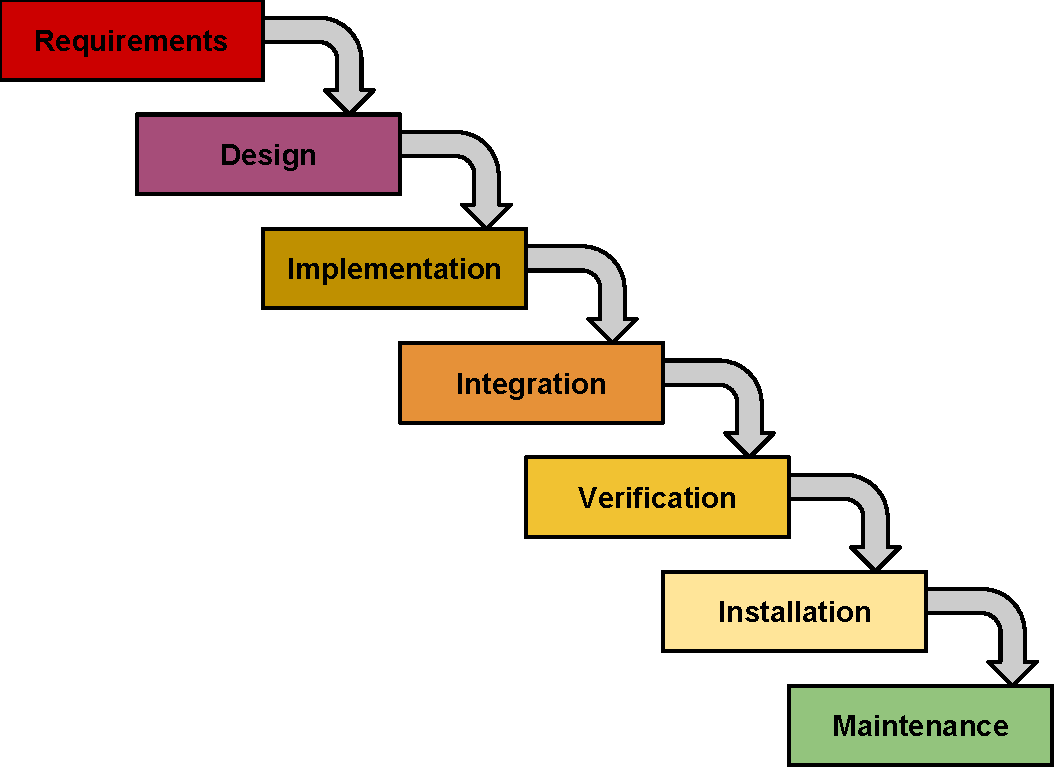
\includegraphics[scale=0.6]{../Figures/Waterfall-model.pdf}
\end{center}
\caption{Development cycle in Waterfall}
\label{figure:waterfall-model}
\end{figure}

The model is easily understandable, structured, and disciplined.
%The clear distinction between project phases make it easier to monitor the progress of the project.
%it can be very hard to adapt to this kind of development model.
However, adopting Waterfall in real software projects can be challenging because it requires to be able to foresee, in the early stages of the project, any problem that could arise later on and plan accordingly.
This is often a very hard task that requires great insight and expertise.

\iffalse
Additionally, each phase of the development cycle is expected to produce a good amount of documentation that will be used for the next phase: documentation is a critical task.
\fi

Waterfall may be suited to large-scale, expensive projects where \'going back\' on design choices is not an option and requirements are clearly established early on and then \'set in stone\'.
However, many software projects nowadays fail to meet these conditions. \cite{WaterfallModel}
% and therefore Waterfall is probably not an appropriate process for them.

%-----------------------------------
%	SUBSECTION 2
%-----------------------------------
\subsection{Scrum Model}
%cite http://www.mountaingoatsoftware.com/agile/scrum

Scrum is an emerging agile development process which is mostly used in software development.
The Scrum approach, which could be described as both iterative and incremental, consists of multiple sprints which last from two to four weeks. 
Sprints begin with a planning meeting and conclude with a review meeting.

%Each sprint is focusing on a set of concrete goals that are in the sprint backlog.
%The sprint backlog consists of tasks that are chosen from the product backlog. 
%They are usually chosen in the sprint planning meeting that is performed before each sprint.
%The product backlog consists of all the features the product should contain, and is usually made in the
%initial phase of the project. It can however be changed and adjusted during the development of the product.
During the sprint planning meeting team members produce a \emph{sprint backlog}: an artifact which defines a set of concrete goals of the sprint and can be seen basically as a \'to-do\' list tasks to be performed.
Such tasks, which in Scrum's terminology are called \emph{stories} are taken from the \emph{product backlog} which is a prioritized list of the requirements of the product.
Although a product backlog is usually made during the early stages of the project, it is subject to change in order to accommodate new or modified requirements. 
The person in charge of populating and ordering the product backlog is the \emph{product owner}.

Each day in a sprint begins with a meeting called \emph{daily scrum}. 
During this meeting which is usually brief, everybody shares the work accomplished since the last daily scrum and their plan for the day, mentioning eventual problems if any. 
A sprint concludes with a sprint \textit{review meeting} where the team evaluates the work done.

%If there are any problems the Scrum master is responsible to resolve the problem.
The whole process is supervised by the \textit{Scrum master} who has the responsability to help other team members to perfom at their best and solve problems that might arise during the process.
Figure \ref{figure:scrum-workflow} shows the workflow in Scrum. \cite{Compendium}

\begin{figure}[h]
\begin{center}
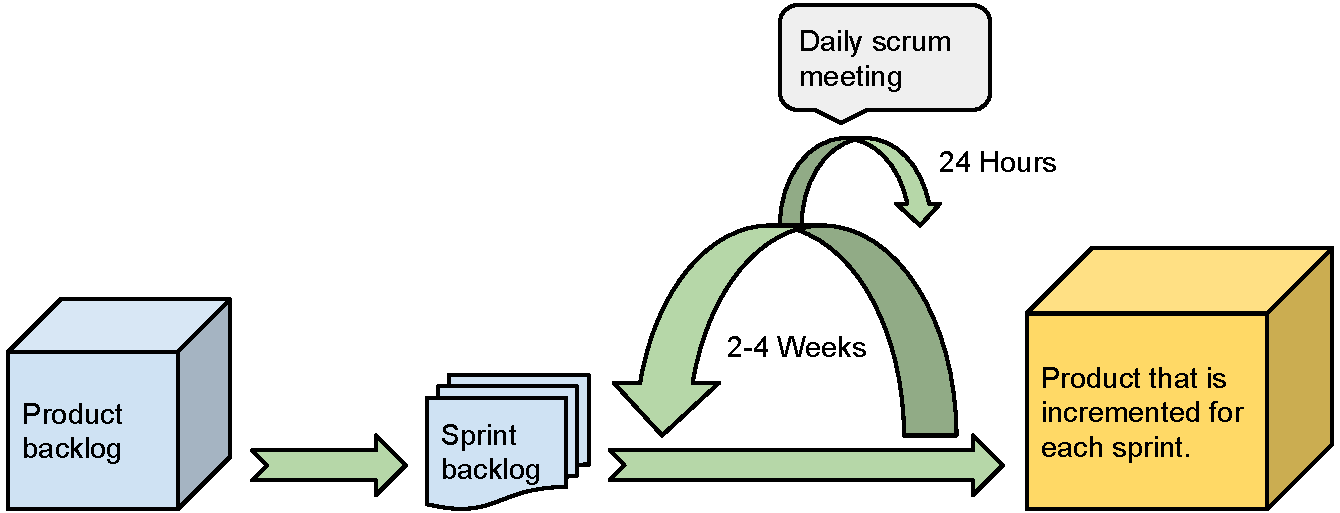
\includegraphics[scale=0.5]{../Figures/Scrum-workflow.pdf}
\end{center}
\caption{Scrum workflow}
\label{figure:scrum-workflow}
\end{figure}

%-----------------------------------
%	SUBSECTION 3
%-----------------------------------
\subsection{Conclusion}
\label{subsec:devprocess}

%Chosing a development process was one of the first tasks of this project.
%We took into consideration many factors such as team size, project scope, time resources.
After discussing about possible alternatives, we decided to use Scrum based on the following considerations:

\begin{enumerate}
\item we didn't have a formal set of requirements from the beginning and we expected their nature to be volatile, that is, subject to change throughout the duration of the project.

%\item at the beginning of the project, our knowledge of both the problem and the technologies involved was limited
%thus it would have been very risk to make design decisions we couldn't adjust later.
%it was highly likely that our design choices in the early phases of the project had to be adjusted multiple times
%before becoming acceptable.
%didn't understand the problem completely, and might have done some wrong
%design decisions in the first phase of the project.

\item at the beginning of the project, our knowledge of both the problem and the technologies involved was limited thus it would have been very risky to make decisions we wouldn't be able to adjust later.

\item given the size of the project and of our group, we wanted a development process with a small overhead. Waterfall is notoriously not a process with a small overhead.

\item we had previous working experiences with Scrum, whereas our experience with Waterfall was only theoretical.

\item the customer hinted us to use an agile method.

\end{enumerate}

All in all, Scrum seemed to fit very well the nature of this project.
We thought that iterating the same activities over and over would have led to a natural improvement of our process and left a lot of possibilities to adjust the requirements and thus the design accordingly.

However, we made some adjustment to the process in order to adapt it to our specific case.

\textbf{Daily scrum}\newline
We performed daily scrum on days we planned to work together: Mondays and Wednesdays.
Because everyone in the group had to attend courses, or to deliver assignments, or a job, or all these things, we couldn't work every day on the project. 
Since there was nothing to report, we didn't see the need for a daily scrum meeting.

\textbf{Sprint review meetings}\newline
Usually this meeting is held at the end of a sprint. 
In our case however, because our last meeting each week was on Wednesdays but we often worked on the project later during the rest of the week, we decided to combine the sprint review meeting with the sprint planning meeting (on Mondays every two weeks).

%The Scrum master would prepare a sprint backlog, and receive the informal approval of the customer.

%With the Scrum method it is also a lot easier to adjust the project direction if we are going down the wrong path.
%Our customer also advised us to use an agile method as our development methodology.
%We thought that scrum would be a good methodology as it is a widely known and respected development process in the programming community.
%The ability to change the design and choices we had made earlier in the project was very important to us.
%If we for example were to make a choice that the customer wasn't pleased with, we would have the ability to fix the problem in the next sprint.
%This would have been very hard to do in a non agile development methodology like the waterfall model.


\section{Existing Solutions}
\label{section:existing-solutions}

This section describes existing solutions which have helped us get a better overview of technologies and design patterns used to solve this kind of problem. 
What we present in this section are the ones we found most relevant and inspiring for our work.

%The following technologies were a good inspiration source and help in our project,
%as they already were similar or did contain components that our application also would contain.

%-----------------------------------
%	SUBSECTION 1
%-----------------------------------
\subsection{HealthVault}
%http://msdn.microsoft.com/en-us/healthvault/jj128027

HealthVault is Microsoft's online platform to collect, store and monitor personal health information. %It offers a single, central repository of a person's health.
One of its most interesting features is interoperability with third-party solutions which are, in HealthVault terminology and in this subsection hereafter, referred to as \textit{Apps}.

Examples of Apps include:
\begin{itemize}
\item smartphone and desktop applications
\item devices like step counters, blood glucose meters, weighting scales\ldots
\item third-party health services like Withings, \ldots
\end{itemize}

At the moment of writing, HealthVault supports more than 300 applications and 80 devices (in the U.S.).
Apps are used to populate a user's health record by collecting health measurements and parameters and, in turn, make use of such information to provide services.
In order to connect to HealthVault, third-party applications need to be authorized by the user upon first use. 
Authorization can be restricted to a specific set of data: e.g. an App may be authorized to access weight and glucose records but not others (allergies, pregnancies\ldots).

%See figure \ref{} for a diagram showing the different authentication and authorization steps.

Interoperability is achieved through an XML-over-HTTP API which, together with several software development kits (SDK) for major mobile platforms and languages enables developers to build HealthVault-enabled applications with ease.

In HealthVault a single data measurement is called \textit{thing}.
Basically, a \textit{thing} represents a measurement of some health parameter e.g. heart rate, weight.
\textit{Things} are represented using XML, see an example below (a weight \textit{thing}).

\begin{lstlisting}[language=XML]
<weight>
  <value>
    <kg>60</kg>
    <display units="kg">132</display>
  </value>
  <when>
    <date>
      <y>1990</y>
      <m>1</m>
      <d>1</d>
    </date>
    <time>
      <h>1</h>
      <m>0</m>
      <s>0</s>
    </time>
  </when>
</weight>
\end{lstlisting}

%The devices might be weighting scales, step counters, blood glucose monitors and more.
%While the applications can be different types of mobile, tablet or desktop apps.
%It is also possible to share the information stored in HealthVault with e.g. family members or a doctor.
%It's possibile to selectively share health information with other
%people which could be family doctors or relatives.

Additionally, HealthVault supports exporting of data in industry-standard formats and storage of medical imaging formats such as \textit{DICOM}. 
The services provides a good degree of availability and redundancy. \cite{HealthVault}

\begin{figure}[h]
\begin{center}
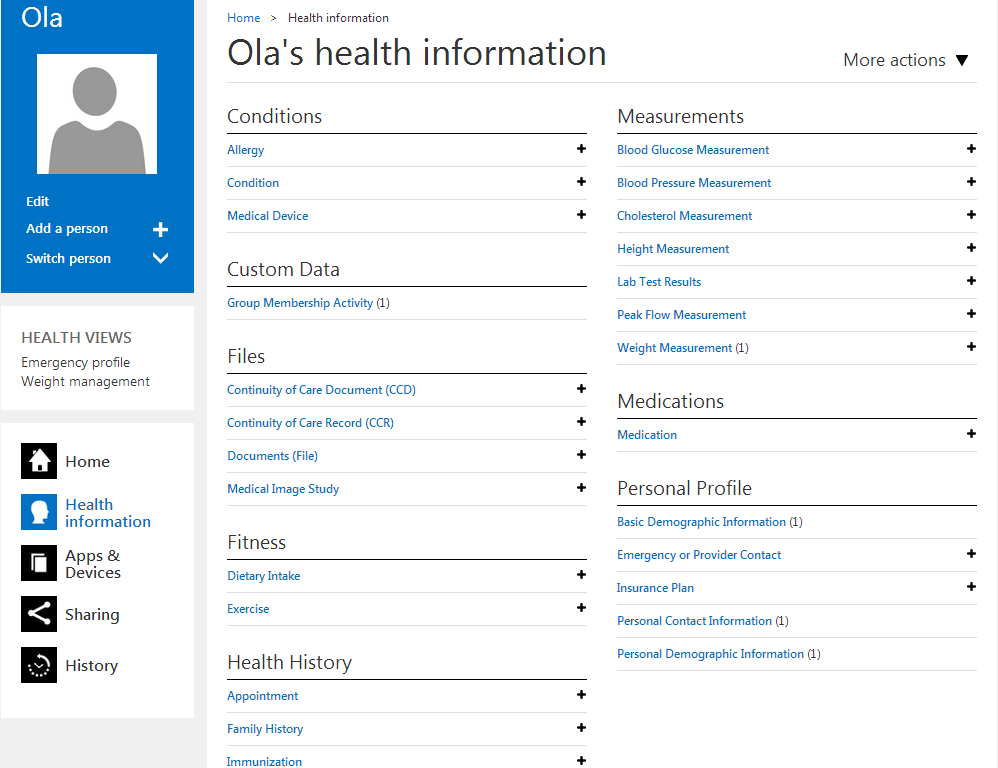
\includegraphics[scale=0.50]{../Figures/hv-page.png}
\end{center}
\caption{HealthVault web interface}
\label{figure:hv-page}
\end{figure}

%maybe we cant use this picture. it's good tho...
\iffalse
\begin{figure}[h]
\begin{center}
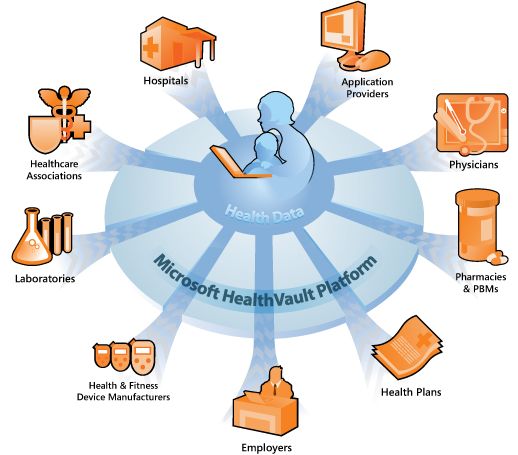
\includegraphics[scale=0.6]{../Figures/hv-cloud.png}
\end{center}
\caption{HealthVault apps}
\label{figure:hv-apps}
\end{figure}
\fi

%An HealthVault account can be linked to multiple individuals.

%-----------------------------------
%	SUBSECTION 2
%-----------------------------------
\subsection{human/api}
\label{section:humanapi}

The human/api is a RESTful web API for health data developed by human/api Inc.
Its aim is to offer a single access point to people's health information in order to facilitate developing health applications.
For this purpose, human/api collects people's health parameters (blood pressure, weight\ldots) from a variety of third-party services (e.g. Withings) and devices (e.g. sensors) and normalizes it.
The data is then made available through a clean and well documented web API.
This has the benefit of providing a single service for application developers to authenticate against in order to obtain users' health information, without having to integrate with multiple services individually.
Additionally, all data is represented using standardized models and format (JSON) of which we present an example below. \cite{HumanAPI}

%They have an API that contains multiple different well defined JSON strings for different kinds of human related data.
%Each JSON string contains all the necessary information that is needed to represent each type of health data.
%For example heart rate is defined by an id, user id, time, value and unit in the following way:

%See below an example of an blood pressure measurement as represented in human/api using JSON.

\begin{lstlisting}[language=JSON]
{
  "id": "string",
  "userId": "string",
  "time": "date",
  "value": {
    "diastolic": "int",
    "systolic": "int",
    "unit": "string"
  },
  "heartRate": "int"
}
\end{lstlisting}

%-----------------------------------
%	SUBSECTION 3
%-----------------------------------
\subsection{android-heart-rate-monitor}
\label{subsec:hr}

android-heart-rate-monitor is an open source (Apache 2.0 license) Android application that can be used to measure the user heart rate. 
The application uses the phone's camera and flash to compute \'redness\' levels on user's fingertips. 
These are supposed to increase in correspondence with heartbeats.
The application computes an average \'redness\' value and uses that to detected heartbeats and calculate a beats per minute (BPM) measurement. \cite{AndroidHeartRateMonitor}

%According to the author, it takes around thirty seconds to get an accurate reading.
%It measures the heart rate of the user with help of the camera and flash light on the phone.

%-----------------------------------
% SUBSECTION 4
%-----------------------------------
\subsection{Open eHealth Foundation}

The goal of Open eHealth Foundation is to create and share open source software components for the healthcare ICT industry.
One of their products is an integration platform called Open eHealth Integration Platform (IPF).
It is based on Apache Camel and has support for connecting systems in the eHealth domain. \cite{OpenEHealthFoundation}


%-----------------------------------
%	SUBSECTION 5
%-----------------------------------
\subsection{Conclusion}

The solutions presented in this subsection were of great influence in our work.
\verb|human/api| influenced our data models and representation as well as being a good example of how to implement security.
HealthVault, together with its SDKs proved to be a valuable example of a modern health integration platform.
We made use of HealthVault SDK to interact with the Microsoft's platform and were able to re-use a large portion of the code shipped as example.

%Our integration platform needs to send and receive information. 
%With help of the Human API we found out how the structure of this information should be.
The android-heart-rate-monitor application was used to provide functionality that would have taken some effort to implement from scratch.
% starting point for creating the heart rate application that we needed in our project.



\section{Security concerns}

\subsection{HIPAA - Health Insurance Portability and Accountability Act}

After discussing security with the customer we brought up the topic of HIPAA \cite{HIPAA}. 
Even though there is no similar act in Norway the customer believed that taking a starting point from HIPAA to discuss the security in NIPEN would be a smart basis. 

\subsubsection{Storage of data}
When the data is at rest the network should be protected from intrusions.
The hard drives where the data is stored must be encrypted. \cite{Encryption}
HIPAA does not specify what type of encryption should be used, they only specify that it should be encrypted.

\begin{figure}[H]
\centering
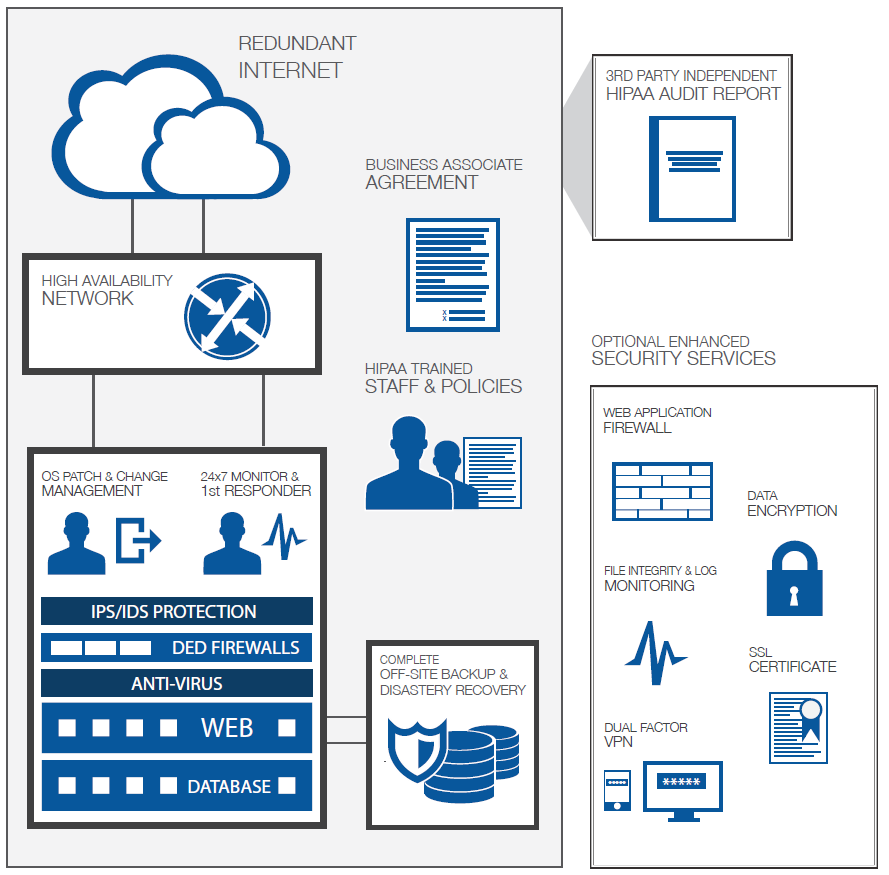
\includegraphics[scale=0.50]{../Figures/hipaa.png}
\caption{HIPAA Compliant Data Center Architecture from www.onlinetech.com}
\label{figure:HIPAA}
\end{figure}

\subsubsection{Transportation of data}
In HIPAA the transportation of data is described that it needs to use Secure Socket Layer. 
This layer is designed to give communication security over the Internet. \cite{SSL}

\subsubsection{Authentication}
There are multiple systems already in use today in Norway for authenticating users. 
Some of the biggest systems are MinId, BankID, Buypass and Commfides.
The most widespread right now is BankId, with almost 3 million users as of this writing\footnote{\href{https://www.bankid.no/}{https://www.bankid.no/}}.
It would be worth a consideration to use BankID to authenticate the citizens. 
The reason behind this is that it is a widespread system and something the citizens are familiar with. 

When considering what type of authentication the medical professionals should use there are multiple factors to consider. 
Ease of use, efficiency and be able to make an audit trail are some extra factors too consider.
It might be as successful to develop a separate system of authenticating the health professionals if BankID turns out to be cumbersome and unable to be used in the different situations needed for this system. 
For HIPAA there needs to be a system to know which information was accessed, when, and by whom. \cite{Audit}

\subsubsection{Giving data to third party systems}
Not only should this system accept data from third parties. 
There should also be functionality for exporting data from the system to third party providers. 
For this to happen there needs to be a system for the end users, the citizens, to understand where and to whom the data is going.
Any data that is Protected Health Information \cite{PHI}, which is defined as any data classified as health information connected by the patients identifiers, the end user must control how this information is shared. 
In the end its up to the user who they want to share their data with.
What could be smart is to introduce a Norwegian certification so that the end user knows that the data providers they want to export their data to follows the rules mentioned in previous subsections. 
That way it is easier for the user to trust new systems with their sensitive data.

\subsection{OAuth 2.0}

OAuth 2.0 is a protocol that could potentially be used for our integration platform.
OAuth 1.0 is outdated, and hence we will mainly focus on OAuth 2.0 in this section.
What this protocol does is that it grants third party applications partial access to a system.
In our case this could for example be only access to the API concerning heart rates or weights in NIPEN.

%\subsection{What is OAuth?}

Many applications want to have access to an API provider to gain access to a users information.
However, the user doesn't always want to give his/hers credentials to these applications.
Lets say that a user wants to have an application that is able to upload images to his/hers facebook account.
The user doesn't want to give the application the credentials for facebook.
This would be highly insecure, since once the application has the authentication information of a user it is able to do whatever it wants with the account.
To handle this we need some kind of protocol, this is where OAuth comes in.
With OAuth we are able to give a third party application partial access to a system without handing over the credentials of a user.
This is a token based system, where the application receives a token which grants it access to use some of the systems services.

When a third party app wants to use a system that uses OAuth, it first needs to be registered in that system.
Under registration the system usually wants some basic information about the application.
This might include name of the application, a description, logo and etc.
A redirect URI also needs to be registered.
This URI needs to use TLS, i.e. must begin with \textit{https}.
This address is used to send an authentication token from the system to the application.
After the registration, the application should receive a client ID which is used to identify the application at the system.

Now users should be able to connect the application with theirs account on the system.
The way it works is that through the application they will be sent to a website of the system the application wants to connect with.
There the user will be asked if he/she wants to grant permissions to the application.
If the user agrees, then he/she will be redirected to the applications specified redirect URI with an access token as a parameter.
The application will now use this token to access the system.
When the user doesn't want the application to have access to the system any more, he/she can simply disallow the applications access through the systems website.

An example of how OAuth works is given in figure \ref{figure:oauth-in-a-nutshell}.
In this example we see a website that wants to send images to a users facebook account.
If the user allows the application access through facebook, then facebook will send an access token to the website.
Then \textit{www.ImageToFacebook.com} is able to send images to the users account, where the access token is used for authentication.
The user should be able to disallow the website access at any time on facebooks website. \cite{OAuth}

\begin{figure}[h]
\centering
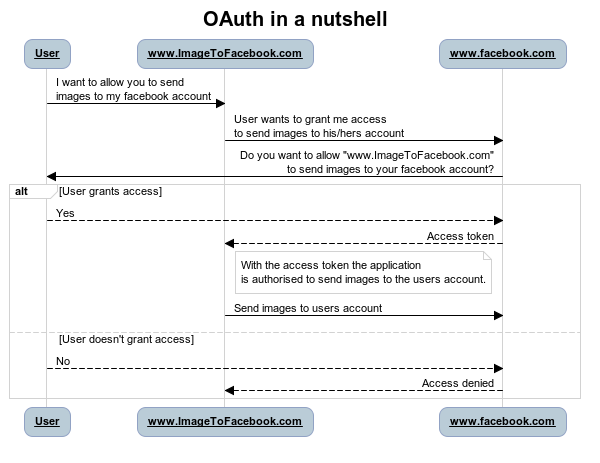
\includegraphics[scale=1.0]{../Figures/oauth-in-a-nutshell.png}
\caption{OAuth in a nutshell}
\label{figure:oauth-in-a-nutshell}
\end{figure}


%----------------------------------------------------------------------------------------
%	SECTION 4
%----------------------------------------------------------------------------------------
\section{Used Technologies}
\label{section:used-technologies}

This section contains the technologies we used in our project.
We are going to go through what type of technologies we used for the server (back-end), web page (front-end), database and for the development of applications for mobile units. 
It also contains some other technologies that were needed in the project.

%-----------------------------------
%	SUBSECTION 1
%-----------------------------------
\subsection{Server}

\textbf{Java}

Java is a general-purpose programming language, which means that it can be used in a wide variety of application domains.
It is platform independent, and thus makes it easy to develop software for different operation systems.
Web programming is one of the domains that Java is used for, hence makes it possible to write a service that runs in the back-end of a website.
The web services created with Java allows creating a bridge between the database and the front-end. 
This makes it possible to create a communication between the user and the database at the server. \cite{Java}

\textbf{Spring Framework}

The Spring Framework is an open source application framework and inversion of control container for Java. 
We use the Spring framework to set up a RESTful service and to handle the data access from the database. \cite{SpringFramework1}\cite{SpringFramework2}

\textbf{Apache Tomcat}

Apache Tomcat is an implementation of the JSP (JavaServer Pages) and Java Servlet technologies.
It makes it possible to deploy and run a website with its services on a server.
Numerous industries and organizations use the Tomcat server as it has support for large-scale and mission-critical web applications. \cite{ApacheTomcat}

%-----------------------------------
%	SUBSECTION 2
%-----------------------------------
\subsection{Database}

\textbf{MySQL}

MySQL is one of the most widely used relational database management system.
The MySQL Community Edition is open source and freely available.
It is developed to handle large databases, support many users at the same time and it is also scalable.
It makes it possible to store and retrieve data in an efficient and structured manner. \cite{MySQL}

\textbf{MySQL Workbench}

MySQL Workbench is a free-to-use tool which allows to easily manage MySQL databases.
We used MySQL Workbench for database design and deployment both locally (for testing) and remotely (production).


%-----------------------------------
%	SUBSECTION 3
%-----------------------------------
\subsection{Website}

\textbf{HTML5}

HTML is the standard World Wide Web's markup language, where HTML5 is the newest HTML version as of this writing.
It is used to structure and visualize web pages on the internet.
By writing a document with HTML a web browser is later on able to interpret the document and visualize it in a structured manner. \cite{HTML5}

\textbf{CSS3}

CSS describes the look and format of a document written in HTML.
It allows one to use different fonts, colors and adjust the layout of a web page.
By using CSS and separating it from the HTML, it is possible to allow multiple pages share the same style.
Thus it is easier to maintain and adapt the web pages to different environments through CSS. \cite{CSS3}

\textbf{Bootstrap}

Bootstrap contains HTML and CSS templates for web designers.
This makes it easier to make a good looking web page without putting too much effort into the design. \cite{Bootstrap}

\textbf{JavaScript}

JavaScript is an interpreted computer programming language that runs in the browser of the user.
It is allowed to make changes in the HTML DOM, interact with the user, control the browser and communicate asynchronously.
Since it can communicate with the server asynchronously, it makes the web page more dynamic.
What this means is that a web page can acquire new information and change the site without reloading. \cite{JavaScript}

\textbf{jQuery}

jQuery is a JavaScript library for manipulating and traversing the HTML DOM.
All the features jQuery contains are also possible to do with pure JavaScript, but jQuery helps the developer to
implement the different features in an easier way.
For example it contains predefined methods for event handling and animation.
It also makes it easier to communicate with the server through AJAX. \cite{jQuery}

\textbf{Chart.js}

Chart.js is a JavaScript library for creating graphs and charts.
It helps the developer to visualize data through different types of graphs in an easy manner.
The library has support for different types of two dimensional data, e.g. value per time.
It also has the ability to display multiple graphs in the same chart.  \cite{Chartjs}

%-----------------------------------
%	SUBSECTION 4
%-----------------------------------
\subsection{Mobile Technologies}

\textbf{Android SDK}

Android SDK contains the tools necessary for developing, debugging and testing an Android app.
With the SDK it is possible to write and modify applications for an Android phone. \cite{AndroidSDK}

%-----------------------------------
%	SUBSECTION 5
%-----------------------------------
\subsection{Other Technologies}

\textbf{Maven}

Maven is a software tool for managing a programming project.
It has the ability to build and compile programming code based on the content of a POM (Project Object Model) file.
It keeps track of all the frameworks used, and is able to download them before building the project. \cite{Maven}

\textbf{Git}

Git is a version control system that is free and open source.
This is an important tool to keep track of all the changes made to the source code, it also makes it easier for multiple developers to work on the same source.
Git makes it easy to roll back changes made to the code, in case something was wrongly implemented.
It also has the possibility to divide the project into different branches.
Which means that the code can be copied into multiple different places, and developed separately in cases where trying out different solutions is necessary.
If a good solution is made, the branch can later on be merged together with the main branch.
It is also possible to have a branch for release versions and a development branch. \cite{Git}

%-----------------------------------
%	SUBSECTION 6
%-----------------------------------
\subsection{Conclusion}

We chose the technologies specified above based on our earlier experience and what we found most appropriate for our solution.
Before we started this project we discussed our competencies.
This was of great help in choosing the right technologies that were going to be used.
Most of us already had some different degree of experience in most of the technologies mentioned above.
This made it much easier for us to chose the right set of frameworks and languages to work with.
For example from table \ref{table:competencies} we can see that all of us were very familiar with Java, Git and SQL.
This made it clear for us to use those technologies.

%----------------------------------------------------------------------------------------
%	SECTION 5
%----------------------------------------------------------------------------------------
\section{Testing}
\label{section:testing}

%In this section we are going to go through some of the testing frameworks used in our project.
In this section we are going to go through some of the testing frameworks explored during our preliminary study.

\subsection{JUnit}

JUnit is a Java framework for writing tests. It is also a good tool when using test driven development.
With help of this framework it is possible to write tests for different parts of the code, then check if it runs as it should.
It is also possible to use JUnit with Maven.
When doing so it will first run all the tests, and if the tests are successful the application will be executed. \cite{JUnit}

\subsection{Jasmine}

Jasmine is a framework for testing JavaScript code.	
It doesn't require a DOM and is also not dependent on any other frameworks. \cite{Jasmine}

\subsection{Conclusion}

When using test driven development it is important to have some frameworks for testing the code.
New bugs are often introduced to applications when extending it with new functions and features.
With help of the technologies mentioned above it is much easier to find the new bugs, and hence fix them quicker.